\documentclass{article}
\usepackage{graphicx}
\usepackage[a4paper, hmargin = 2.5cm, vmargin = 2.5cm]{geometry}
\usepackage[english]{babel}

\title{Database project : Travel agency \\ (Milestone 1)}
\author{Oliver Baltisberger, Rachid Flueckiger, Christian Pernet}
\date{\today}

\begin{document}
	\maketitle
	
	\section*{Project description}
	Our project aims to implement a database for a simple customer relationship management 
	for a travel agency. 
	Several travel agencies employ collaborators. These employees sell trips to 
	customers. 
	In our example, the trips are organized trips. They also have a begin date, a 
	duration, a price and a category. 
	The category can be e.g. cruse, road trip, safari, ...
	
	\section*{Queries examples}
			
			\begin{enumerate}
				\item List all employees and the number of trips they have 
							sold in the last 12 months.
				\item Make a list of all employees working at a 
							particular branch office.
				\item Which employee has sold most trips?
				\item Sales made by an employee. 
				\item Make a list of the clients.
				\item List all clients by number of trips bought.
				\item Make a list of the clients who have reserved a trip.
				\item Make a list of all clients that have booked the same accomodation 
							during a defined period.
				\item Make a list of the trips to a specific city/country. 
				\item Make a list of the trips sold during a defined period.
				\item What is average duration/price of a trip?
				\item What is the preferred payment method for trips?
				\item List most popular months of travel (e.g. more 
							trips in July than in November).
				\item Make a list of all accomodations in a country/city. 
				\item Make a list of all accomodation types 
							(e.g. hotel, vacation homes).
				\item What is the most popular accomodation (type) during a 
				      defined period?
				\item What type of accomodation/transport/activity 
							types are most popular?
	
				\end{enumerate}	
				
	\hrule
	\vspace{2 cm}
	On the next page, you find the ER-Diagram of this project. 
	
	
	\newpage
	
	\section*{ER-Diagram}
	\begin{figure}[htbp]
		\centering
			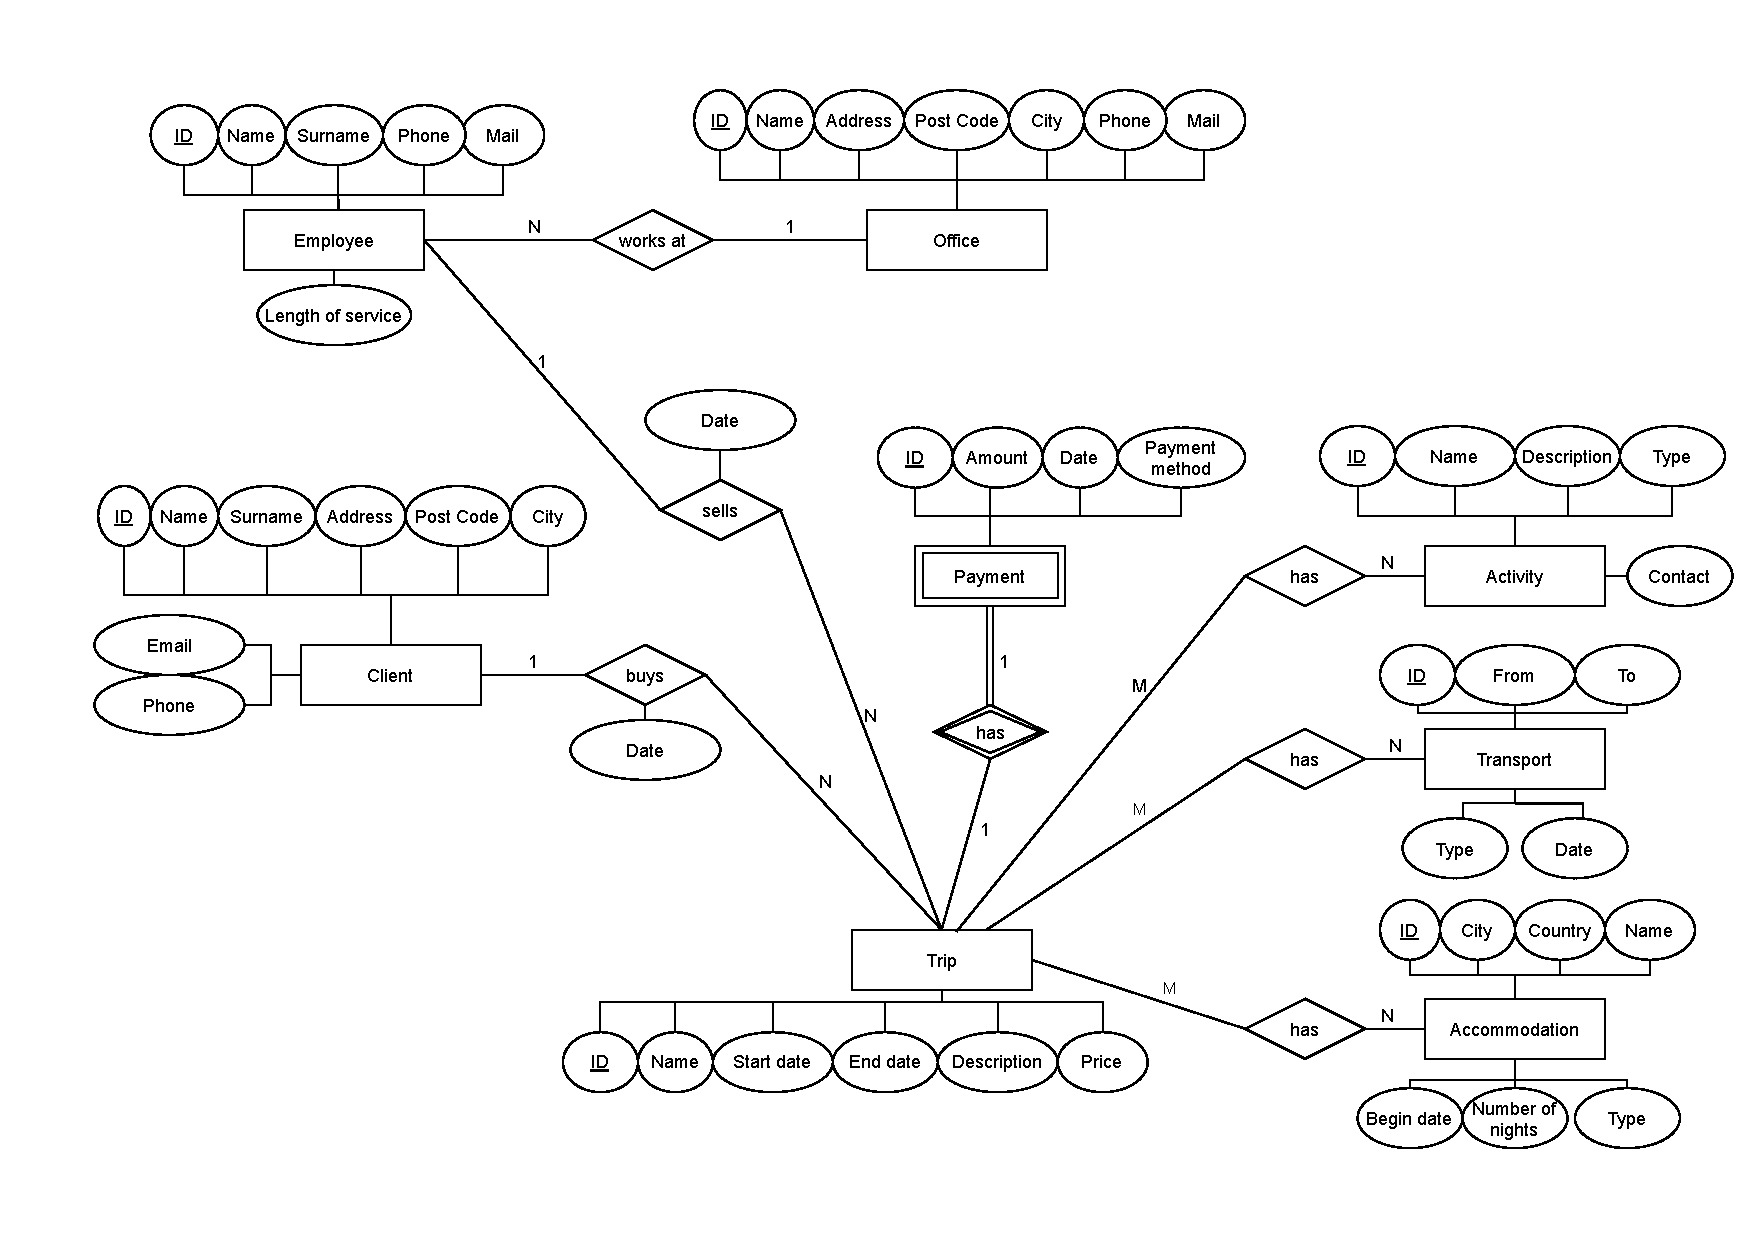
\includegraphics[width=1.15\textwidth, angle=90]{../Proposition 2.pdf}
		\label{ER-Model}
		\caption{Travel agency ER-Model}
	\end{figure}
	

\end{document}